\begin{enumerate}[label=\thesubsection.\arabic*,ref=\thesubsection.\theenumi]
	\item  Find the vector equation of the line passing through $\myvec{1&2&3}^{\top}$ and parallel to the planes $\myvec{1&-1&2}\vec{x} = 5$ and $\myvec{3&1&1}\vec{x} = 6$.  
		\\
    \solution
		The direction vector of the line  is given by 
\begin{align*}
 \myvec{1&-1&2 \\ 3&1&1}\vec{m} = 0
 \xleftrightarrow[]{R_2\rightarrow -\frac{3}{4}{R_1} + \frac{1}{4}{R_2}} \myvec{1&-1&2 \\ 0&1&-\frac{5}{4}}\\
   \myvec{1&-1&2 \\ 0&1&-\frac{5}{4}} \xleftrightarrow[]{R_1\rightarrow {R_1} + {R_2}} \myvec{1&0&\frac{3}{4} \\ 0&1&-\frac{5}{4}}
   \\
 \implies \vec{m} =\myvec{-3\\5\\4}
\end{align*}
$\therefore$ the equation of the line is
\begin{align}
    \vec{x} = \myvec{1\\2\\3} + \lambda\myvec{-3\\5\\4} 
\end{align}


	\item Find the equation of the plane with an intercept 3 on the Y-axis and parallel to ZOX-Plane.\\
    \solution
		\iffalse
\documentclass[A4,12pt,twocolumn]{IEEEtran}
%
\usepackage{setspace}
\usepackage{gensymb}
%\doublespacing
\singlespacing

%\usepackage{graphicx}
%\usepackage{amssymb}
%\usepackage{relsize}
\usepackage[cmex10]{amsmath}
%\usepackage{amsthm}
%\interdisplaylinepenalty=2500
%\savesymbol{iint}
%\usepackage{txfonts}
%\restoresymbol{TXF}{iint}
%\usepackage{wasysym}
\usepackage{amsthm}
%\usepackage{iithtlc}
\usepackage{mathrsfs}
\usepackage{txfonts}
\usepackage{stfloats}
\usepackage{bm}
\usepackage{cite}
\usepackage{cases}
\usepackage{subfig}
%\usepackage{xtab}
\usepackage{longtable}
\usepackage{multirow}
%\usepackage{algorithm}
%\usepackage{algpseudocode}
\usepackage{enumitem}
\usepackage{mathtools}
\usepackage{steinmetz}
\usepackage{tikz}
\usepackage{circuitikz}
\usepackage{verbatim}
\usepackage{tfrupee}
\usepackage[breaklinks=true]{hyperref}
%\usepackage{stmaryrd}
\usepackage{tkz-euclide} % loads  TikZ and tkz-base
%\usetkzobj{all}
\usetikzlibrary{calc,math}
\usepackage{listings}
    \usepackage{color}                                            %%
    \usepackage{array}                                            %%
    \usepackage{longtable}                                        %%
    \usepackage{calc}                                             %%
    \usepackage{multirow}                                         %%
    \usepackage{hhline}                                           %%
    \usepackage{ifthen}                                           %%
  %optionally (for landscape tables embedded in another document): %%
    \usepackage{lscape}     
\usepackage{multicol}
\usepackage{chngcntr}
%\usepackage{enumerate}

%\usepackage{wasysym}
%\newcounter{MYtempeqncnt}
\DeclareMathOperator*{\Res}{Res}
%\renewcommand{\baselinestretch}{2}
\renewcommand\thesection{\arabic{section}}
\renewcommand\thesubsection{\thesection.\arabic{subsection}}
\renewcommand\thesubsubsection{\thesubsection.\arabic{subsubsection}}

\renewcommand\thesectiondis{\arabic{section}}
\renewcommand\thesubsectiondis{\thesectiondis.\arabic{subsection}}
\renewcommand\thesubsubsectiondis{\thesubsectiondis.\arabic{subsubsection}}

% correct bad hyphenation here
\hyphenation{op-tical net-works semi-conduc-tor}
\def\inputGnumericTable{}                                 %%

\lstset{
%language=C,
frame=single, 
breaklines=true,
columns=fullflexible
}
%\lstset{
%language=tex,
%frame=single, 
%breaklines=true
%}

\begin{document}
%


\newtheorem{theorem}{Theorem}[section]
\newtheorem{problem}{Problem}
\newtheorem{proposition}{Proposition}[section]
\newtheorem{lemma}{Lemma}[section]
\newtheorem{corollary}[theorem]{Corollary}
\newtheorem{example}{Example}[section]
\newtheorem{definition}[problem]{Definition}
%\newtheorem{thm}{Theorem}[section] 
%\newtheorem{defn}[thm]{Definition}
%\newtheorem{algorithm}{Algorithm}[section]
%\newtheorem{cor}{Corollary}
\newcommand{\BEQA}{\begin{eqnarray}}
\newcommand{\EEQA}{\end{eqnarray}}
\newcommand{\define}{\stackrel{\triangle}{=}}

\bibliographystyle{IEEEtran}
%\bibliographystyle{ieeetr}


\providecommand{\mbf}{\mathbf}
\providecommand{\pr}[1]{\ensuremath{\Pr\left(#1\right)}}
\providecommand{\qfunc}[1]{\ensuremath{Q\left(#1\right)}}
\providecommand{\sbrak}[1]{\ensuremath{{}\left[#1\right]}}
\providecommand{\lsbrak}[1]{\ensuremath{{}\left[#1\right.}}
\providecommand{\rsbrak}[1]{\ensuremath{{}\left.#1\right]}}
\providecommand{\brak}[1]{\ensuremath{\left(#1\right)}}
\providecommand{\lbrak}[1]{\ensuremath{\left(#1\right.}}
\providecommand{\rbrak}[1]{\ensuremath{\left.#1\right)}}
\providecommand{\cbrak}[1]{\ensuremath{\left\{#1\right\}}}
\providecommand{\lcbrak}[1]{\ensuremath{\left\{#1\right.}}
\providecommand{\rcbrak}[1]{\ensuremath{\left.#1\right\}}}
\theoremstyle{remark}
\newtheorem{rem}{Remark}
\newcommand{\sgn}{\mathop{\mathrm{sgn}}}
\providecommand{\abs}[1]{\left\vert#1\right\vert}
\providecommand{\res}[1]{\Res\displaylimits_{#1}} 
\providecommand{\norm}[1]{\left\lVert#1\right\rVert}
%\providecommand{\norm}[1]{\lVert#1\rVert}
\providecommand{\mtx}[1]{\mathbf{#1}}
\providecommand{\mean}[1]{E\left[ #1 \right]}
\providecommand{\fourier}{\overset{\mathcal{F}}{ \rightleftharpoons}}
%\providecommand{\hilbert}{\overset{\mathcal{H}}{ \rightleftharpoons}}
\providecommand{\system}{\overset{\mathcal{H}}{ \longleftrightarrow}}
	%\newcommand{\solution}[2]{\textbf{Solution:}{#1}}
\newcommand{\solution}{\noindent \textbf{Solution: }}
\newcommand{\cosec}{\,\text{cosec}\,}
\providecommand{\dec}[2]{\ensuremath{\overset{#1}{\underset{#2}{\gtrless}}}}
\newcommand{\myvec}[1]{\ensuremath{\begin{pmatrix}#1\end{pmatrix}}}
\newcommand{\mydet}[1]{\ensuremath{\begin{vmatrix}#1\end{vmatrix}}}
%\numberwithin{equation}{section}
\numberwithin{equation}{subsection}
%\numberwithin{problem}{section}
%\numberwithin{definition}{section}
\makeatletter
\@addtoreset{figure}{problem}
\makeatother

\let\StandardTheFigure\thefigure
\let\vec\mathbf
%\renewcommand{\thefigure}{\theproblem.\arabic{figure}}
\renewcommand{\thefigure}{\theproblem}
%\setlist[enumerate,1]{before=\renewcommand\theequation{\theenumi.\arabic{equation}}
%\counterwithin{equation}{enumi}


%\renewcommand{\theequation}{\arabic{subsection}.\arabic{equation}}

\def\putbox#1#2#3{\makebox[0in][l]{\makebox[#1][l]{}\raisebox{\baselineskip}[0in][0in]{\raisebox{#2}[0in][0in]{#3}}}}
     \def\rightbox#1{\makebox[0in][r]{#1}}
     \def\centbox#1{\makebox[0in]{#1}}
     \def\topbox#1{\raisebox{-\baselineskip}[0in][0in]{#1}}
     \def\midbox#1{\raisebox{-0.5\baselineskip}[0in][0in]{#1}}

\vspace{3cm}


\title{GEOMETRY}
\author{Shristy Sharma (EE22BNITS11001)}





% make the title area
\maketitle

\newpage

%\tableofcontents

\bigskip

\renewcommand{\thefigure}{\theenumi}
\renewcommand{\thetable}{\theenumi}
%\renewcommand{\theequation}{\theenumi}


%Download all python codes 
%
%\begin{lstlisting}
%svn co https://github.com/JayatiD93/trunk/My_solution_design/codes
%\end{lstlisting}

%Download all and latex-tikz codes from 
%
%\begin{lstlisting}
%svn co https://github.com/gadepall/school/trunk/ncert/geometry/figs
%\end{lstlisting}
%


\section{PROBLEM 1}
SOLUTION:\\
\fi
The normal vector to the ZOX plane is
\begin{align} 
\vec{n} = \myvec{0\\1\\0}.
\end{align}
Since, Y-axis has the intercept 3, the desired plane passes through the point
\begin{align}
\vec{P}=\myvec{0\\3\\0}.
\end{align}
Thus, the equation of the plane is given by,
\begin{align}
	\vec{n}^\top \brak{\vec{x}-\vec{P}} &= 0\\
	\implies \myvec{0&1&0} \vec{x}&= 3
\end{align}
See Fig. 
     \ref{fig:chapters/12/11/3/8/1}.
\begin{figure}[h!]
  \centering
   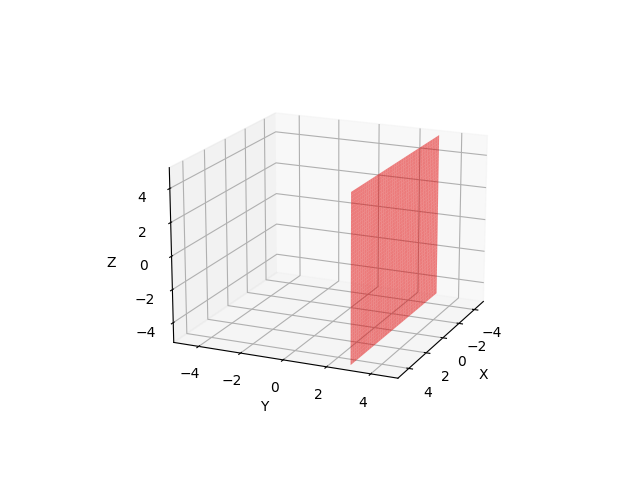
\includegraphics[width=\columnwidth]{chapters/12/11/3/8/figs/plane1.png}
    \caption{}
     \label{fig:chapters/12/11/3/8/1}
     \end{figure}  

\item Find the equation of the line  parallel to the line $3x-4y+2=0$ and passing through the point (-2,3).
\label{chapters/11/10/3/7}
\\
\solution 
\iffalse
% #######################################
% ########### FILL THESE IN #############
% #######################################
\def\mytitle{MATRICES}
\def\mykeywords{}
\def\myauthor{GOWTHAMI MANDAVA}
\def\contact{gowthamimandava999@gmail.com}
\def\mymodule{ Future Wireless Communication(FWC22012)}
% #######################################
% #### YOU DON'T NEED TO TOUCH BELOW ####
% #######################################
\newcommand{\myvec}[1]{\ensuremath{\begin{pmatrix}#1\end{pmatrix}}}
\let\vec\mathbf
\providecommand{\pr}[1]{\ensuremath{\Pr\left(#1\right)}}
\providecommand{\qfunc}[1]{\ensuremath{Q\left(#1\right)}}
\providecommand{\sbrak}[1]{\ensuremath{{}\left[#1\right]}}
\providecommand{\lsbrak}[1]{\ensuremath{{}\left[#1\right.}}
\providecommand{\rsbrak}[1]{\ensuremath{{}\left.#1\right]}}
\providecommand{\brak}[1]{\ensuremath{\left(#1\right)}}
\providecommand{\lbrak}[1]{\ensuremath{\left(#1\right.}}
\providecommand{\rbrak}[1]{\ensuremath{\left.#1\right)}}
\providecommand{\cbrak}[1]{\ensuremath{\left\{#1\right\}}}
\providecommand{\lcbrak}[1]{\ensuremath{\left\{#1\right.}}
\providecommand{\rcbrak}[1]{\ensuremath{\left.#1\right\}}}
\documentclass[10pt, a4paper]{article}
\usepackage[a4paper,outer=1.5cm,inner=1.5cm,top=1.75cm,bottom=1.5cm]{geometry}
\twocolumn
\usepackage{circuitikz}
\usepackage{amsmath,bm}
\usepackage{amsthm}
\usepackage{mathtools}
\usepackage{amsfonts}
\usepackage{amssymb}
\usepackage{graphicx}
\graphicspath{{./images/}}
%colour our links, remove weird boxes
\usepackage[colorlinks,linkcolor={black},citecolor={blue!80!black},urlcolor={blue!80!black}]{hyperref}
%Stop indentation on new paragraphs
\usepackage[parfill]{parskip}
%% Arial-like font
\usepackage{lmodern}
\renewcommand*\familydefault{\sfdefault}
%Napier logo top right
\usepackage{watermark}
%Lorem Ipusm dolor please don't leave any in you final report ;)
\usepackage{karnaugh-map} 
\usepackage{tabularx}
\usepackage{lipsum}
\usepackage{xcolor}
\usepackage{listings}
%give us the Capital H that we all know and love
\usepackage{float}
%tone down the line spacing after section titles
\usepackage{titlesec}
%Cool maths printing
\usepackage{amsmath}
%PseudoCode
\usepackage{algorithm2e}

\titlespacing{\subsection}{0pt}{\parskip}{-3pt}
\titlespacing{\subsubsection}{0pt}{\parskip}{-\parskip}
\titlespacing{\paragraph}{0pt}{\parskip}{\parskip}
\newcommand{\figuremacro}[5]{
    \begin{figure}[#1]
        \centering
        \includegraphics[width=#5\columnwidth]{#2}
        \caption[#3]{\textbf{#3}#4}
        \label{fig:#2}
    \end{figure}
}


 \lstset{
frame=single, 
breaklines=true,
columns=fullflexible
}

\thiswatermark{\centering \put(1,-110){\includegraphics[scale=0.05]{IIT_logo.jpg}} }
\title{\mytitle}
\author{\myauthor\hspace{1em}\\\contact\\IITH\hspace{0.5em}-\hspace{0.5em}\mymodule}
\date{}
\hypersetup{pdfauthor=\myauthor,pdftitle=\mytitle,pdfkeywords=\mykeywords}
\sloppy
% #######################################
% ########### START FROM HERE ###########
% #######################################
\begin{document}
 \maketitle
 \tableofcontents
 
    
 

 
    
    
    
 
 \Large\section{Problem}
 \fi
\\
\solution 
\iffalse
 \section{Solution}
 \begin{center}
 Given equation is 3x-4y+2=0
\\the parallel line passing through point(-2,3)
\begin{align}
\textbf{n}^{\top}(\textbf{x}-\textbf{p})=0 
\end{align}
\label{tab:truthtable}
    \setlength{\arrayrulewidth}{0.2mm}
\setlength{\tabcolsep}{5pt}
\renewcommand{\arraystretch}{1.25}
    \begin{tabular}{|c|c|}
    \hline % <-- Alignments: 1st column left, 2nd middle and 3rd right, with vertical lines in between
      \large\textbf{Symbol} & \large\textbf{Co-ordinates} \\
      \hline
       \large \textbf{n} & $\ \begin{pmatrix} 3\\ -4 \end{pmatrix}$  \\
       \hline
       \large p & $\ \begin{pmatrix} -2\\ 3 \end{pmatrix}$ \\
       \hline
       	\large c & 2 \\
      \hline
   \end{tabular}
\\ by substituting we get
\fi
From the given information, 
\begin{align}
{\vec{n}}=\myvec{3\\-4} \\
\implies 
	\myvec{3&-4}\cbrak{\vec{x}-\myvec{-2\\3}}&=0
	\\
	&=-18 
\end{align}
which is the required equation of the line.
\iffalse
  therefore,the equation parallel to the given equation and passing through the point(-2,3) is 3x-4y+18=0
 \end{center}
 \section{Plot}
         \centering
        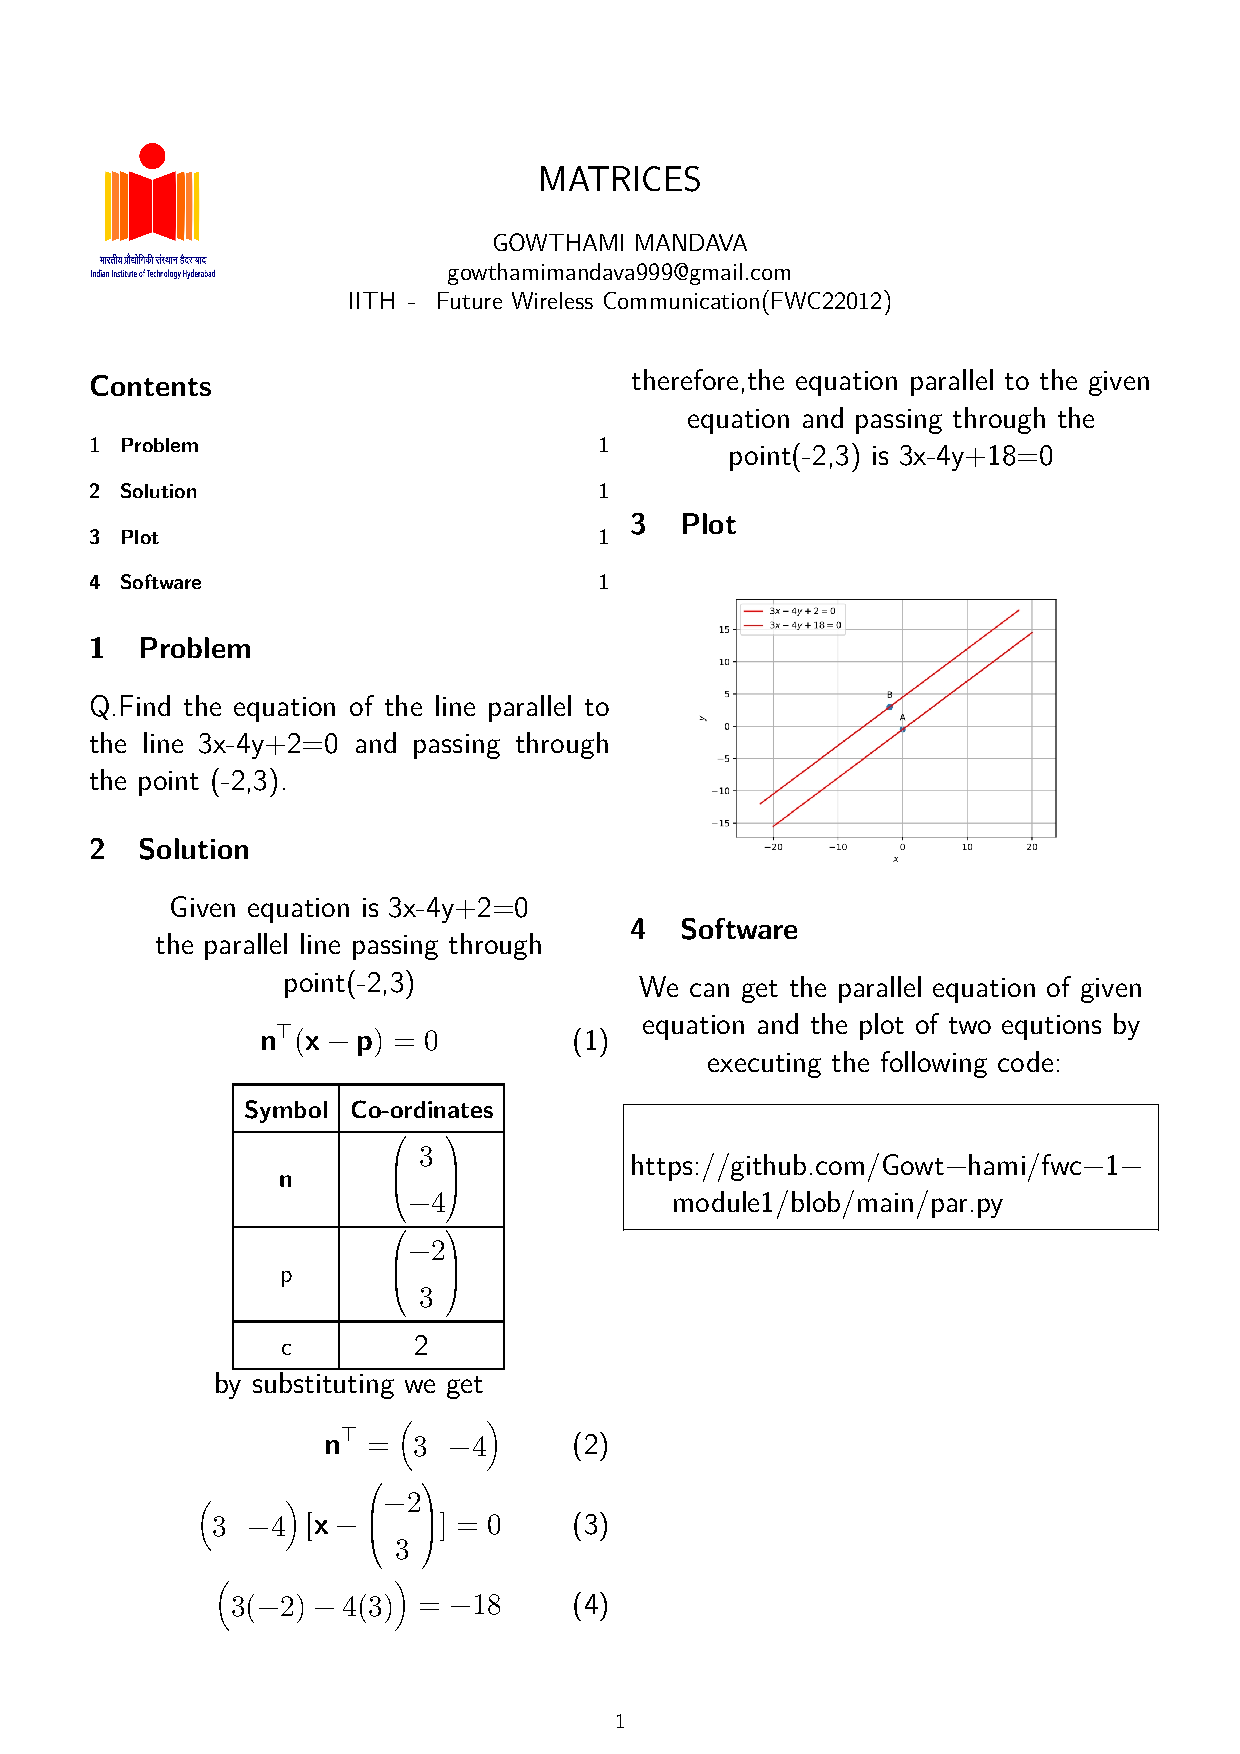
\includegraphics[scale=0.275]{mat.jpg}
  \section{Software}
  We can get the parallel equation of given equation and the plot of two equtions by executing the following code:
 \vspace{3mm} 
\begin{lstlisting}

https://github.com/Gowt-hami/fwc-1-module1/blob/main/par.py
\end{lstlisting}
\end{document}
\fi

\item 
	Find the equation of the line through the point (0,2) making an angle $\frac{2\pi}{3}$ with the positive X-axis. Also find the equation of the line parallel to it and crossing the Y-axis at a distance of 2 units below the origin.
	\\
	\solution
\label{chapters/11/10/2/14}
The equation of the first line is 
\begin{align}
	\myvec{\sqrt{3} &1}\myvec{\vec{x}-\myvec{0\\2}}&=0
	\\
	\implies 
	\myvec{\sqrt{3}&1}
	\vec{x}&=2
\end{align}
The equation of the second line is 
\begin{align}
	\myvec{\sqrt{3} &1}\myvec{\vec{x}-\myvec{0\\-2}}&=0
	\\
	\implies 
	\myvec{\sqrt{3}&1}
\vec{x}=-2
\end{align}
See
		\figref{fig:11/10/2/14}.
	\begin{figure}[!ht]
		\centering
 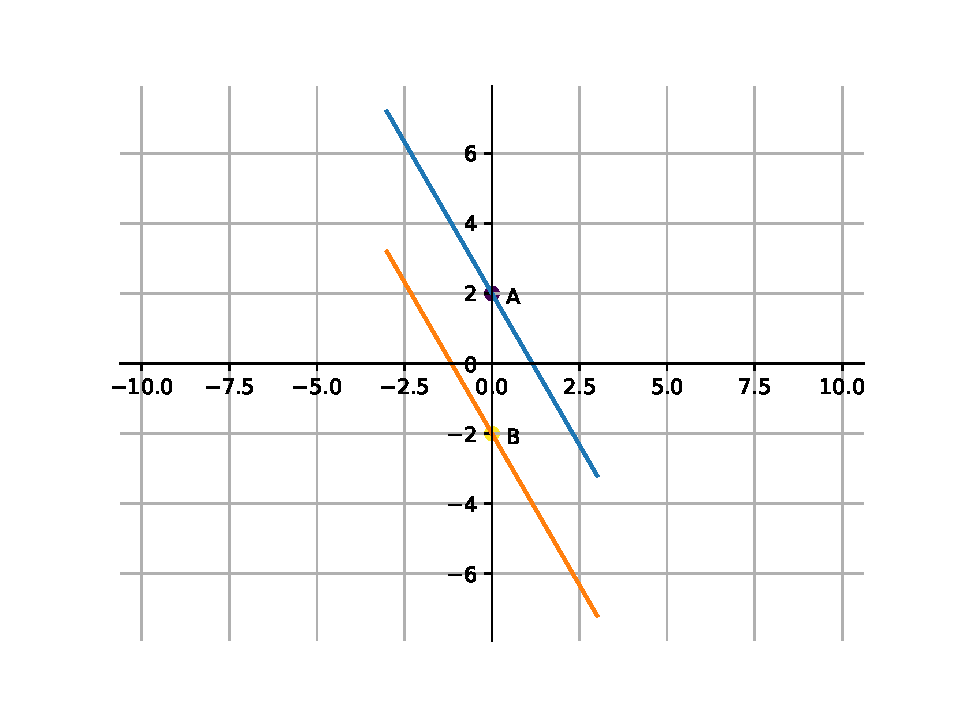
\includegraphics[width=\columnwidth]{chapters/11/10/2/14/figs/fig.pdf}
		\caption{}
		\label{fig:11/10/2/14}
  	\end{figure}

\item  Find the vector equation of the line which is parallel to the vector $3\hat{i}-2\hat{j}+6\hat{k}$ and passes through the point $(1,-2,3)$.
\item Find the equations of the line passing through the point $(3,0,1)$ and parallel to the planes $x+2y=0$ and $3y-z=0.$
\item The equation of a line, which is parallel to $2\hat{i}+\hat{j}+3\hat{k}$ and passes through the point $(5,-2,4)$ is $\dfrac{x-5}{2}=\dfrac{y+2}{-1}=\dfrac{z-4}{3}$.
\item The value of $\lambda$ for which the vectors $3\hat{i}-6\hat{j}+\hat{k}$ $\text{and}$,  $2\hat{i}-4\hat{j}$+$\lambda\hat{k}$ are parallel is
	\begin{enumerate}
			\setlength{\itemsep}{1ex}
\item $\frac{2}{3}$
\item $\frac{3}{2}$
\item $\frac{5}{2}$
\item $\frac{2}{5}$
	\end{enumerate}	
\item Equation of the line passing through (1,2) and parallel to the line $y=3x-1$ is
\begin{enumerate}
\item $y+2=x+1$
\item $y+2=3(x+1)$
\item $y-2=3(x-1)$
\item $y-2=x-1$
\end{enumerate}
\item  Find the equation of the line which passes through the point $(1,2,3)$ and is parallel to the vector $3\hat{i}+2\hat{j}-2\hat{k}$
\item Find the cartesian equation of the line which passes through the point $(-2,4,-5)$ and parallel to the line given by $ \frac{x+3}{3}=\frac{y-4}{5}=\frac{z+8}{6}$.
\end{enumerate}
